\section{Convergence and Model Quality}\label{sec:evaluation}

This section presents a comprehensive analysis of convergence characteristics and model quality metrics for our layer-wise FP8 training approach compared to baseline precision configurations.

\subsection{Training Loss Convergence}

Our experiments demonstrate that layer-wise FP8 training achieves comparable final loss values to BF16 baseline while maintaining superior training dynamics. Figure~\ref{fig:training_loss} shows the training loss progression across different precision configurations.

\begin{figure}[h]
    \centering
    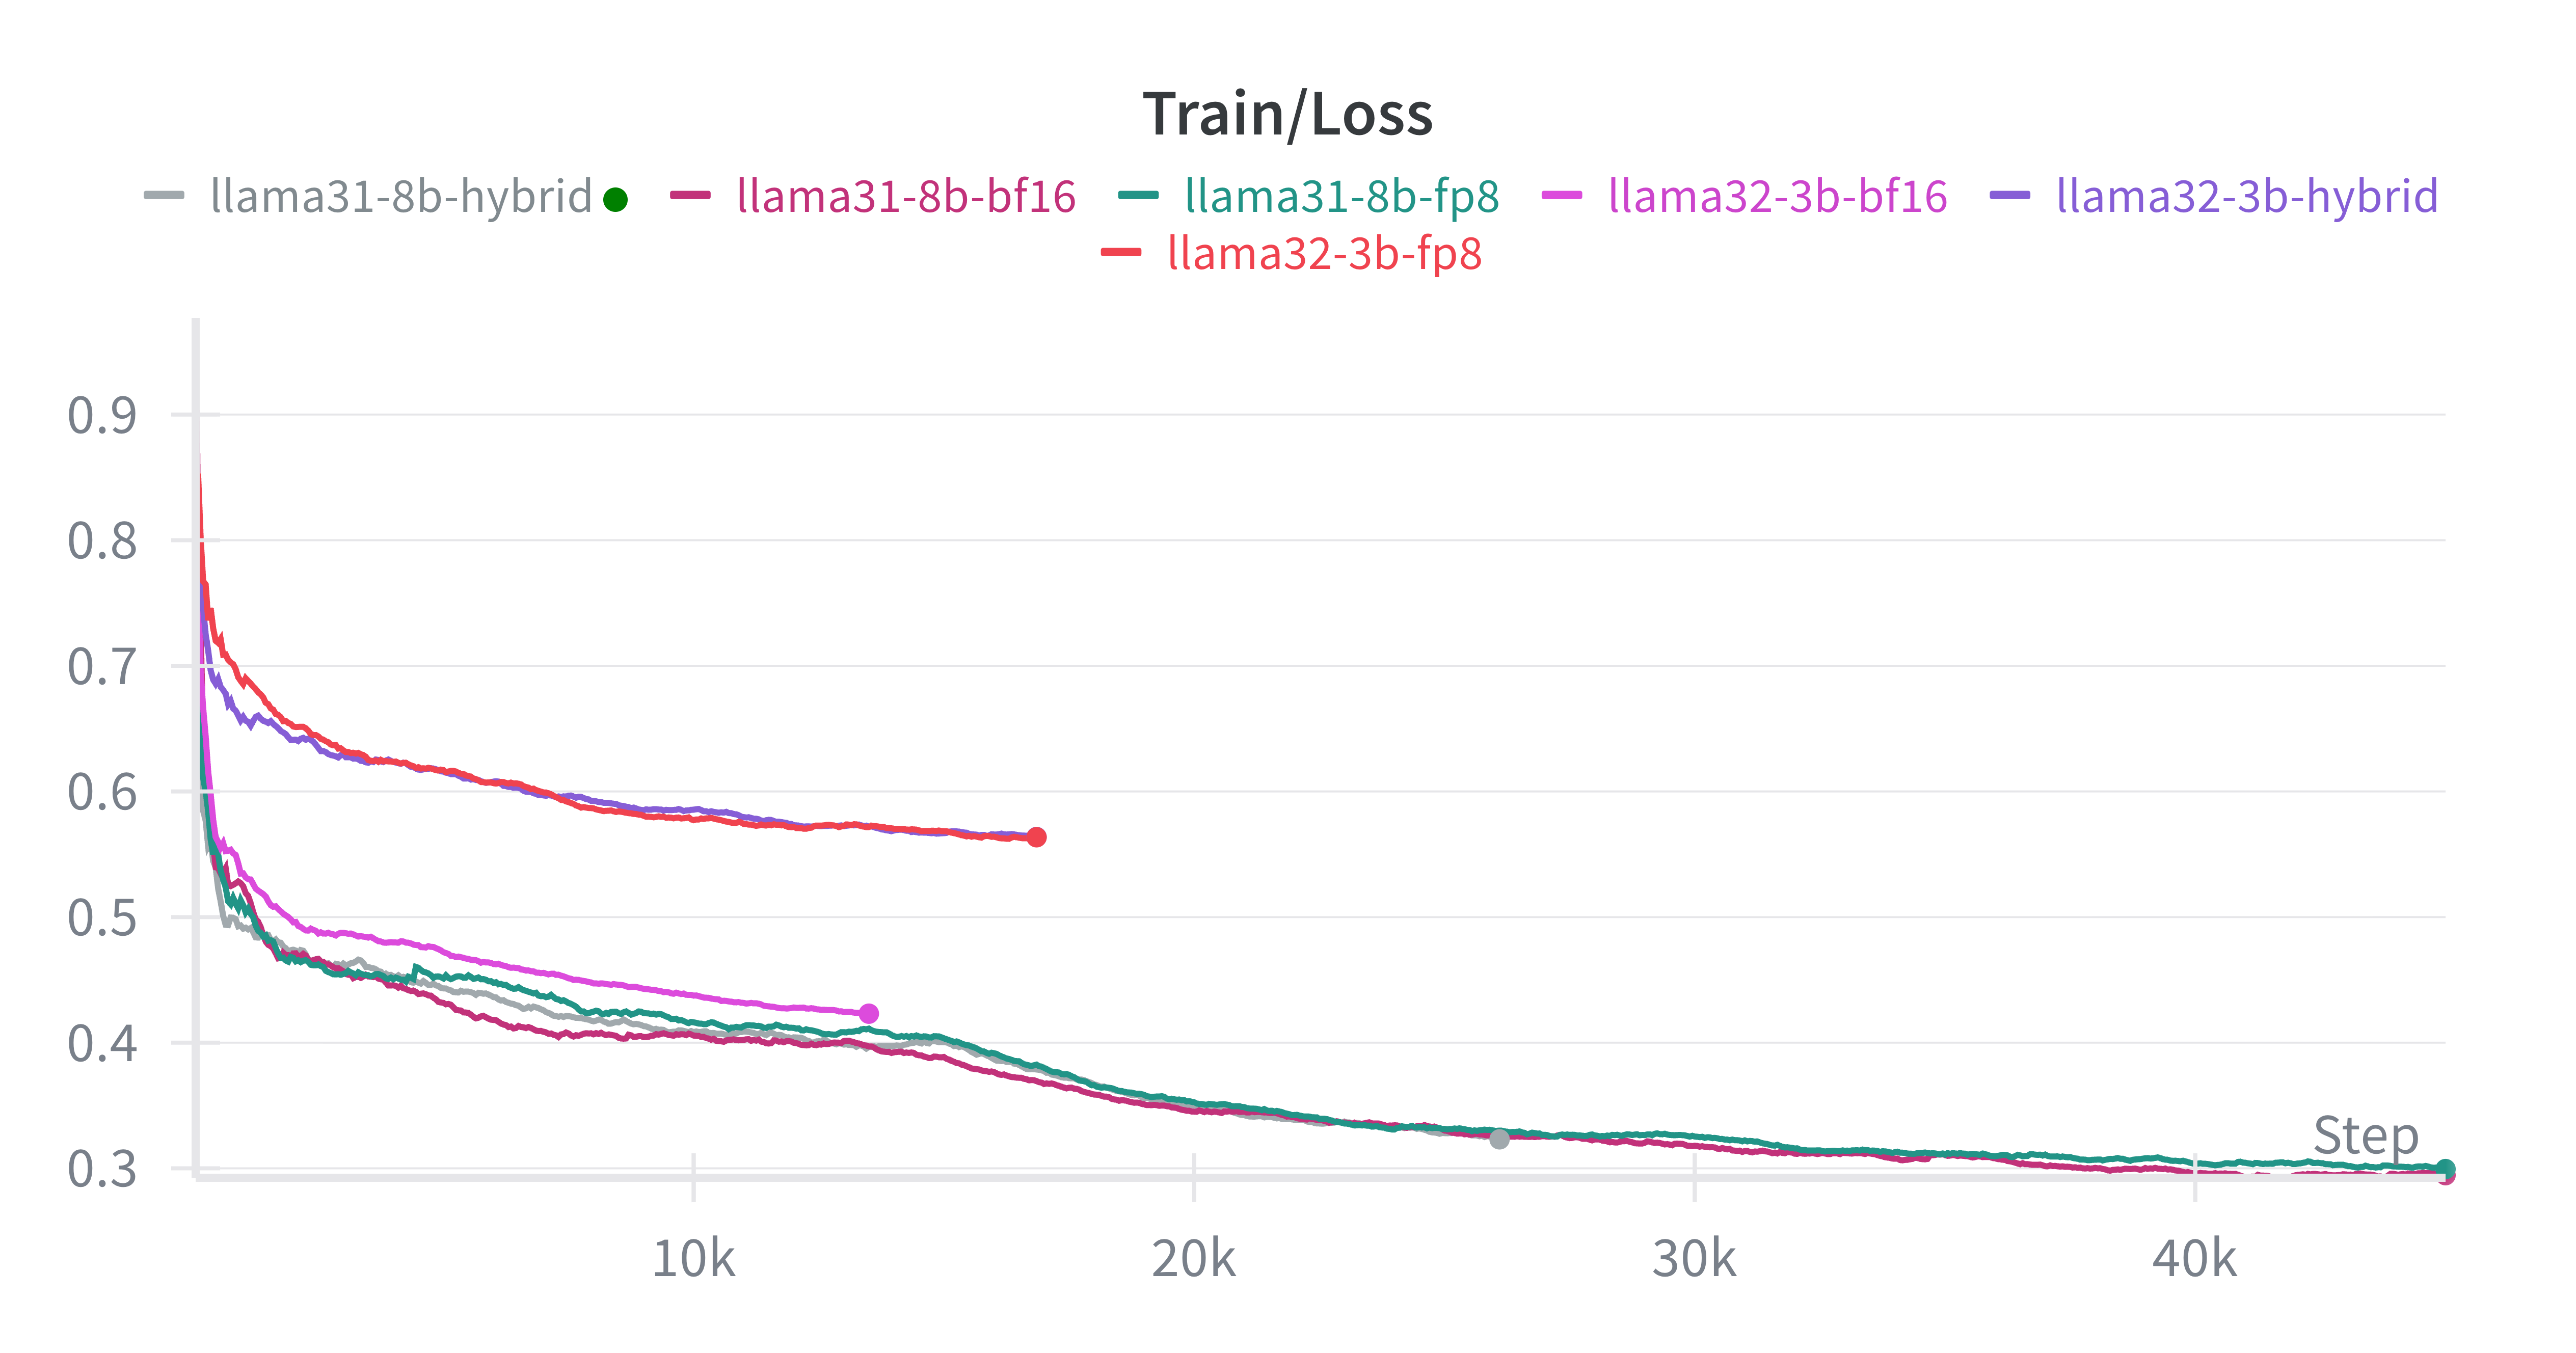
\includegraphics[width=0.9\linewidth]{figures/c4/avg_loss.png}
    \caption{Average training loss comparison between BF16 and FP8 approaches. Both methods demonstrate similar convergence patterns from initial loss of 0.47 to final values below 0.36, with our layer-wise FP8 maintaining smoother dynamics throughout training.}
    \label{fig:training_loss}
\end{figure}

Both BF16 and our FP8 approach converge from initial loss of approximately 0.47 to final values below 0.36 after training. The key distinction lies in convergence stability: our layer-wise format assignment produces smoother loss curves with reduced oscillations compared to hybrid FP8 implementations. This improved stability stems from the selective application of E5M2 format to high-variance components (attention Q/K) while maintaining E4M3 precision for stable operations.

\subsection{Training Perplexity Analysis}

Training perplexity measurements across both model scales confirm that our layer-wise FP8 approach maintains model quality comparable to BF16 baselines. Figure~\ref{fig:training_perplexity} illustrates perplexity values across different model scales and precision formats.

\begin{figure}[h]
    \centering
    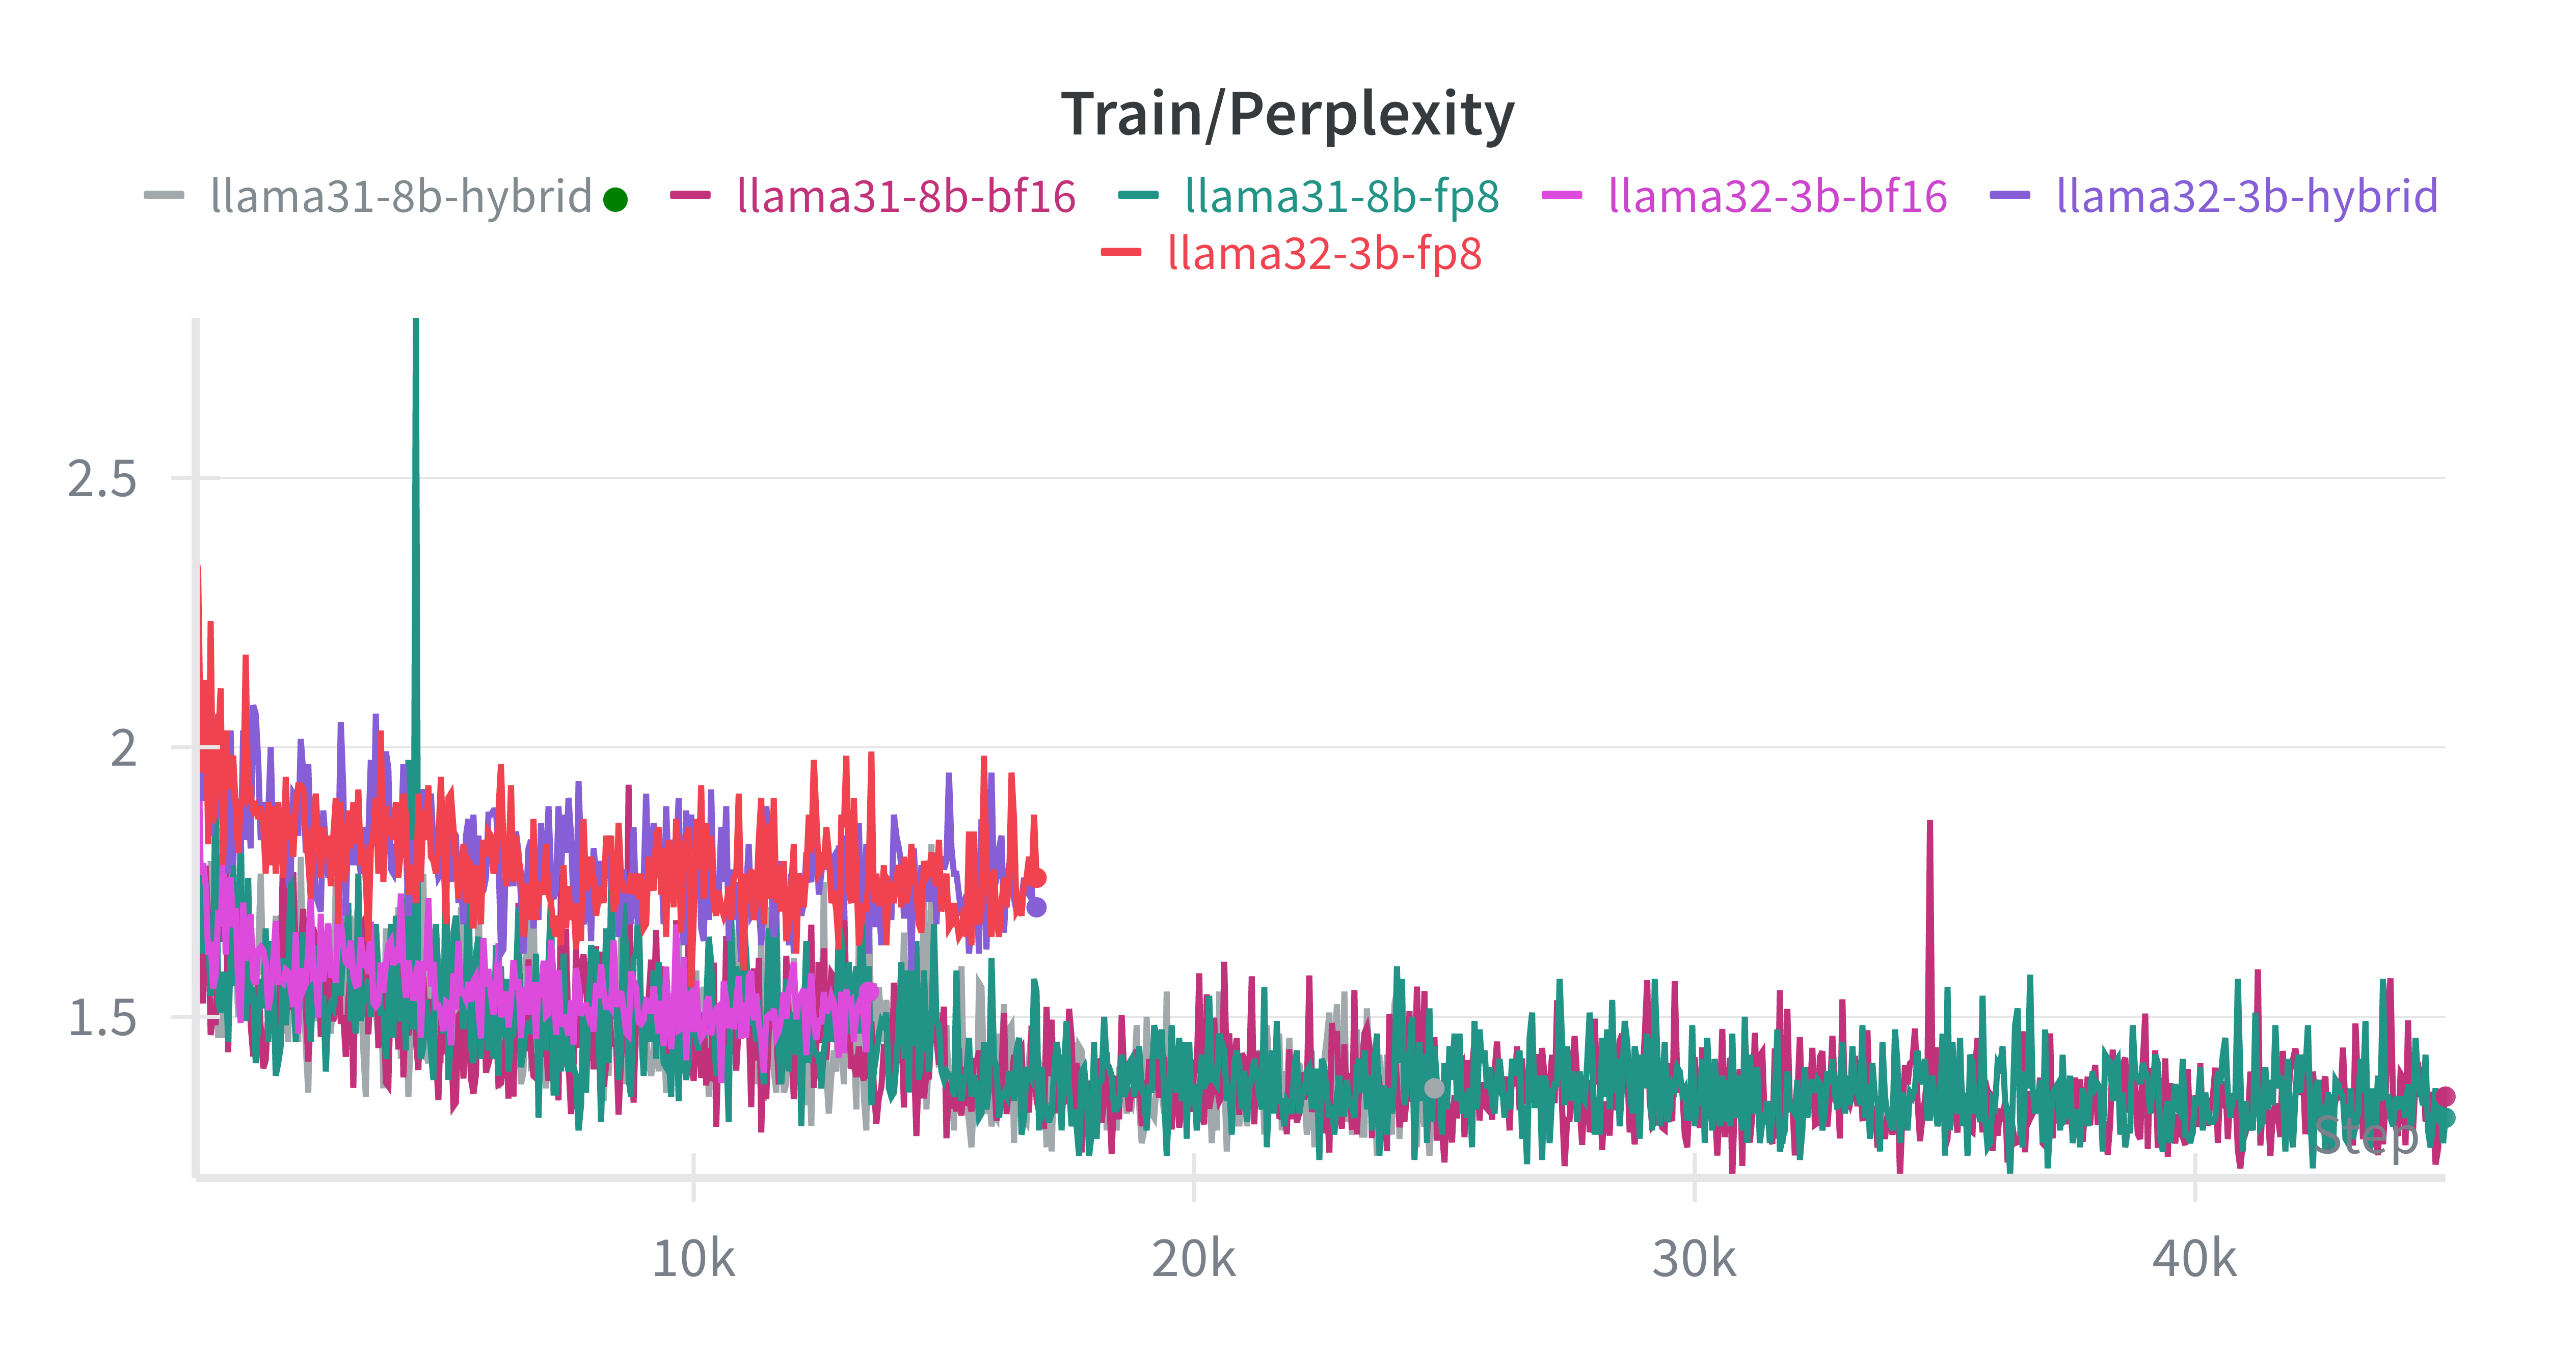
\includegraphics[width=0.9\linewidth]{figures/c4/train_perplexity.png}
    \caption{Training perplexity comparison across model scales and precision formats. Our layer-wise FP8 approach maintains perplexity in the 1.30-1.32 range with superior stability compared to hybrid configurations, demonstrating minimal degradation from BF16 baselines.}
    \label{fig:training_perplexity}
\end{figure}

For both Llama-3.2-3B and Llama-3.1-8B configurations, our method achieves perplexity values in the 1.30-1.32 range, demonstrating minimal degradation from full-precision training. Notably, our approach shows more stable perplexity trajectories compared to hybrid FP8 configurations, which exhibit greater variance during training. This stability advantage translates to more predictable model behavior and reliable convergence characteristics.

\subsection{Scale-Dependent Performance Characteristics}

Our results reveal interesting scale-dependent performance patterns:

\textbf{At 3B scale:} Layer-wise FP8 achieves both memory efficiency (10\% reduction) and training speedup (42\% faster), demonstrating clear advantages across all metrics while maintaining numerical stability.

\textbf{At 8B scale:} While memory usage increases slightly due to implementation overheads, training time benefits become more pronounced (27\% faster than BF16, 13\% faster than Hybrid FP8). This suggests that FP8 optimization benefits scale favorably with model size, particularly for training throughput.

These patterns indicate that layer-wise FP8 format assignment provides consistent improvements that become increasingly valuable as models scale, with training time reductions compensating for any memory overhead at larger scales.